\newpage

\hypertarget{subsec:seekAndFind}{}

\subsection{Seek, and ye shall find \ldots}

EA has a model search function that can be quite handy for large models with thousands of elements and a brain that just can't remember where something is. 

\begin{enumerate}

\item[$\blacktriangleright$]Select ``Model Search Window'' and enter the name of an element you wish to find (Fig.~\ref{fig_search01}).\footnote{You can also
access this window by pressing \texttt{ctrl+alt+A}} 

\begin{figure}[htbp]
\begin{center}
  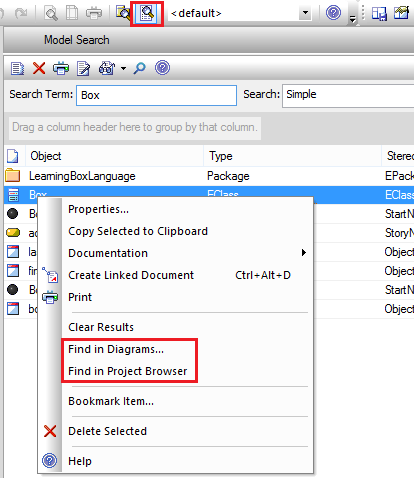
\includegraphics[width=0.63\textwidth]{search1}
  \caption{Model Search Window}  
  \label{fig_search01}
\end{center}
\end{figure}

\item[$\blacktriangleright$] All elements that meet the search criteria are listed and you can right-click on each of the items and select one of the options
above to locate the element.

\item[$\blacktriangleright$] In a similar way, you can locate the corresponding class of an object by right clicking and selecting ``Find/Locate Classifier in
Project Browser.''

\end{enumerate}
